\documentclass[spanish,english]{article}
\usepackage[T1]{fontenc}
\usepackage[a4paper]{geometry}
\geometry{verbose,tmargin=3cm,bmargin=3cm,lmargin=2cm,rmargin=2cm,headheight=2cm,headsep=2cm,footskip=2cm}
\usepackage{float}
\usepackage{amstext}
\usepackage[final]{graphicx}
\usepackage{listings}
\usepackage{xcolor}

\definecolor{codegreen}{rgb}{0,0.6,0}
\definecolor{codegray}{rgb}{0.5,0.5,0.5}
\definecolor{codepurple}{rgb}{0.58,0,0.82}
\definecolor{backcolour}{rgb}{0.95,0.95,0.92}

\lstdefinestyle{Python}{
    backgroundcolor=\color{backcolour},   
    commentstyle=\color{codegreen},
    keywordstyle=\color{magenta},
    numberstyle=\tiny\color{codegray},
    stringstyle=\color{codepurple},
    basicstyle=\ttfamily\footnotesize,
    breakatwhitespace=false,         
    breaklines=true,                 
    captionpos=b,                    
    keepspaces=true,                 
    numbers=left,                    
    numbersep=5pt,                  
    showspaces=false,                
    showstringspaces=false,
    showtabs=false,                  
    tabsize=2
}

\lstset{style=Python}

\usepackage[
backend=biber,
style=numeric,
sorting=ynt
]{biblatex}
\addbibresource{bibliografias.bib}

\makeatletter

%%%%%%%%%%%%%%%%%%%%%%%%%%%%%% LyX specific LaTeX commands.
%% Because html converters don't know tabularnewline
\providecommand{\tabularnewline}{\\}

%%%%%%%%%%%%%%%%%%%%%%%%%%%%%% User specified LaTeX commands.
\usepackage{palatino}
\pagenumbering{gobble}

\makeatother

\usepackage{babel}
\addto\shorthandsspanish{\spanishdeactivate{~<>}}

\begin{document}
\begin{flushleft}
\begin{tabular}{|l|l|}
\hline 
 & \tabularnewline
\textbf{\large{}Instituto Tecnol\'{o}gico de Costa Rica} & QUIZ 3\tabularnewline
\textbf{\large{}Escuela de Computaci\'{o}n} & Entrega: Jueves 16 de Mayo, a trav\'{e}s del TEC digital\tabularnewline
 & Debe subir un \emph{pdf }con la respuesta.\tabularnewline
Programa de Ciencias de los Datos & \tabularnewline
\textbf{Curso: Estadistica} & \tabularnewline
 & \tabularnewline
Profesor: Ph. D. Sa\'{u}l Calder\'{o}n Ram\'{\i}rez & Valor: 100 pts.\tabularnewline
 & Puntos Obtenidos: \_\_\_\_\_\_\_\_\_\_\_\_\tabularnewline
 & \tabularnewline
 & \tabularnewline
 & Nota: \_\_\_\_\_\_\_\_\_\_\_\_\_\_\_\_\tabularnewline
 & \tabularnewline
\cline{2-2} 
\multicolumn{2}{|c|}{}\tabularnewline
\multicolumn{2}{|l|}{Nombre del (la) estudiante: \underline{Yoksan Varela Cambronero}}\tabularnewline
\multicolumn{1}{|l}{} & \tabularnewline
\multicolumn{1}{|l}{} & \tabularnewline
\multicolumn{1}{|l}{} & \tabularnewline
\hline 
\end{tabular}
\par\end{flushleft}
\begin{enumerate}
\item Su equipo tiene por objetivo constuir un modelo Bayesiano que estime
si en 1 mes ser\'{a} necesario que una empresa el\'{e}ctrica necesite
racionar el suministro a sus clientes. Para ello, dado que la empresa
el\'{e}ctrica esta restringida a utilizar solamente fuentes de energ\'{\i}a
renovables (agua y viento), las variables de entrada para predecir
si habr\'{a} cortes el\'{e}ctricos en un mes ($t=1$) o no ($t=0$)
ser\'{a}n la precipitaci\'{o}n $P$ promedio del a\~{n}o hasta ese
mes (medida en $l/m^{2}$ ) y la velocidad del viento $V$ promedio
(medida en $\textrm{km}/h$ ) . Al cabo de un hist\'{o}rico de 5 a\~{n}os,
la empresa el\'{e}ctrica recopil\'{o} los datos en las tablas \ref{tab:Datos-para-la-P}
y \ref{tab:Datos-para-la-P-1}.

\selectlanguage{spanish}%
\begin{table}[H]
\begin{centering}
\begin{tabular}{|c|c|c|c|c|c|c|c|c|c|c|}
\hline 
\selectlanguage{english}%
\selectlanguage{spanish}%
 & \selectlanguage{english}%
$p=400$\selectlanguage{spanish}%
 & \selectlanguage{english}%
$p=500$\selectlanguage{spanish}%
 & \selectlanguage{english}%
$p=600$\selectlanguage{spanish}%
 & \selectlanguage{english}%
$p=700$\selectlanguage{spanish}%
 & \selectlanguage{english}%
$p=800$\selectlanguage{spanish}%
 & \selectlanguage{english}%
$p=900$\selectlanguage{spanish}%
 & \selectlanguage{english}%
$p=1000$\selectlanguage{spanish}%
 & \selectlanguage{english}%
$p=1100$\selectlanguage{spanish}%
 & \selectlanguage{english}%
$p=1200$\selectlanguage{spanish}%
 & \selectlanguage{english}%
$p=1300$\selectlanguage{spanish}%
\tabularnewline
\hline 
\selectlanguage{english}%
$t=0$\selectlanguage{spanish}%
 & \selectlanguage{english}%
5\selectlanguage{spanish}%
 & \selectlanguage{english}%
6\selectlanguage{spanish}%
 & \selectlanguage{english}%
9\selectlanguage{spanish}%
 & \selectlanguage{english}%
11\selectlanguage{spanish}%
 & \selectlanguage{english}%
12\selectlanguage{spanish}%
 & \selectlanguage{english}%
16\selectlanguage{spanish}%
 & \selectlanguage{english}%
18\selectlanguage{spanish}%
 & \selectlanguage{english}%
13\selectlanguage{spanish}%
 & \selectlanguage{english}%
5\selectlanguage{spanish}%
 & \selectlanguage{english}%
2\selectlanguage{spanish}%
\tabularnewline
\hline 
\selectlanguage{english}%
$t=1$\selectlanguage{spanish}%
 & \selectlanguage{english}%
20\selectlanguage{spanish}%
 & \selectlanguage{english}%
13\selectlanguage{spanish}%
 & \selectlanguage{english}%
12\selectlanguage{spanish}%
 & \selectlanguage{english}%
4\selectlanguage{spanish}%
 & \selectlanguage{english}%
2\selectlanguage{spanish}%
 & \selectlanguage{english}%
1\selectlanguage{spanish}%
 & \selectlanguage{english}%
2\selectlanguage{spanish}%
 & \selectlanguage{english}%
1\selectlanguage{spanish}%
 & \selectlanguage{english}%
2\selectlanguage{spanish}%
 & \selectlanguage{english}%
1\selectlanguage{spanish}%
\tabularnewline
\hline 
\end{tabular}\caption{Datos para la variable aleatoria $P$.\label{tab:Datos-para-la-P}}
\par\end{centering}
\selectlanguage{english}%
\selectlanguage{spanish}%
\end{table}
\end{enumerate}

\selectlanguage{spanish}%
\begin{table}[H]
\centering{}%
\begin{tabular}{|c|c|c|c|c|c|c|c|c|c|c|}
\hline 
\selectlanguage{english}%
\selectlanguage{spanish}%
 & \selectlanguage{english}%
$v=5$\selectlanguage{spanish}%
 & \selectlanguage{english}%
$v=10$\selectlanguage{spanish}%
 & \selectlanguage{english}%
$v=15$\selectlanguage{spanish}%
 & \selectlanguage{english}%
$v=20$\selectlanguage{spanish}%
 & \selectlanguage{english}%
$v=25$\selectlanguage{spanish}%
 & \selectlanguage{english}%
$v=30$\selectlanguage{spanish}%
 & \selectlanguage{english}%
$v=35$\selectlanguage{spanish}%
 & \selectlanguage{english}%
$v=40$\selectlanguage{spanish}%
 & \selectlanguage{english}%
$v=45$\selectlanguage{spanish}%
 & \selectlanguage{english}%
$v=50$\selectlanguage{spanish}%
\tabularnewline
\hline 
\selectlanguage{english}%
$t=0$\selectlanguage{spanish}%
 & \selectlanguage{english}%
2\selectlanguage{spanish}%
 & \selectlanguage{english}%
3\selectlanguage{spanish}%
 & \selectlanguage{english}%
5\selectlanguage{spanish}%
 & \selectlanguage{english}%
15\selectlanguage{spanish}%
 & \selectlanguage{english}%
6\selectlanguage{spanish}%
 & \selectlanguage{english}%
3\selectlanguage{spanish}%
 & \selectlanguage{english}%
1\selectlanguage{spanish}%
 & \selectlanguage{english}%
0\selectlanguage{spanish}%
 & \selectlanguage{english}%
0\selectlanguage{spanish}%
 & \selectlanguage{english}%
0\selectlanguage{spanish}%
\tabularnewline
\hline 
\selectlanguage{english}%
$t=1$\selectlanguage{spanish}%
 & \selectlanguage{english}%
22\selectlanguage{spanish}%
 & \selectlanguage{english}%
15\selectlanguage{spanish}%
 & \selectlanguage{english}%
8\selectlanguage{spanish}%
 & \selectlanguage{english}%
3\selectlanguage{spanish}%
 & \selectlanguage{english}%
2\selectlanguage{spanish}%
 & \selectlanguage{english}%
1\selectlanguage{spanish}%
 & \selectlanguage{english}%
0\selectlanguage{spanish}%
 & \selectlanguage{english}%
0\selectlanguage{spanish}%
 & \selectlanguage{english}%
0\selectlanguage{spanish}%
 & \selectlanguage{english}%
0\selectlanguage{spanish}%
\tabularnewline
\hline 
\end{tabular}\caption{Datos para la variable aleatoria $V$.\label{tab:Datos-para-la-P-1}}
\end{table}

\textbf{Nota importante:} Para efectos del desarrollo de este quiz, $t = 0$ se refiere a NO tener que hacer un corte de electricidad y, en su contraparte, $t = 1$ se refiere a que SI se tiene que hacer un corte el\'{e}ctrico.

\begin{enumerate}

\item \textbf{(20 puntos)} Usando pytorch, use el histograma de los datos
anteriores para estimar las densidades $p\left(m_{1}|t=0\right)$,
$p\left(m_{1}|t=1\right),$$p\left(m_{2}|t=0\right)$, $p\left(m_{2}|t=1\right)$.
$m_{1}=p$ (primer dimension) y $m_{2}=v$ (segunda dimension)

Para crear los histogramas solicitados en este punto, se us\'{o} el siguiente c\'{o}digo base, ajustando el tensor y la valor de \textit{t} dependiendo del caso:

\begin{lstlisting}[language=Python]
# Creando el histograma para p(m1|t=0)
# Acomondando los bines para que empiecen en cero
bins = torch.linspace(0, 9, 10)
histogram,bins_hist = torch.histogram(bins,bins=10,weight=P[0,:], density=True)
plt.bar(bins,histogram)
plt.xlabel('Categoria de la Precipitacion')
plt.ylabel('Probabilidades')
plt.title('Histograma para p(m1|t=0)')
plt.show()
\end{lstlisting}

Podemos notar dos cosas importantes en este c\'{o}digo:
\begin{enumerate}
    \item \textbf{El espacio lineal va de 0 a 9:} A pesar de tener diferentes valores num\'{e}ricos para la precipitaci\'{o}n y la velocidad del viento, ambas variables aleatorias tienes 10 diferentes categor\'{i}as o clases. Es por eso que el espacio lineal de los bines va de 0 a 9, dado que estos valores afectan el c\'{a}lculo de la densidad que se explica en el siguiente punto.
    \item \textbf{El uso del par\'{a}metro \textit{density=True} dentro de \textit{torch.histogram}:} Al poner este par\'{a}metro en \textit{True}, el peso de las categor\'{i}as del histograma se normaliza contra los bines, de forma que las barras, en lugar de ser cuentas, son las probabilidades de cada bin. Por lo tanto, con esta opci\'{o}n es que se logr\'{o} mostrar la densidad de probabilidad conditional contra t para cada uno de los casos solicitados en el enunciado.
\end{enumerate}

Con el c\'{o}digo anterior como base se obtuvieron los siguientes histogramas:

\selectlanguage{spanish}%
\begin{figure}[hbtp!]
    \centering
    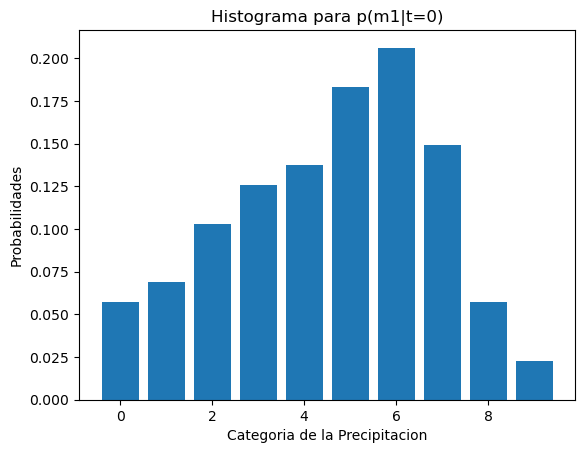
\includegraphics[width=0.75\linewidth]{Quiz_2//Imagenes/histograma_precipitacion_t0.png}
    \caption{Histograma para la precipitaci\'{on} cuando $t = 0$}
    \label{fig:hist_precipitacion_t0}
\end{figure}\newpage

\selectlanguage{spanish}%
\begin{figure}[hbtp!]
    \centering
    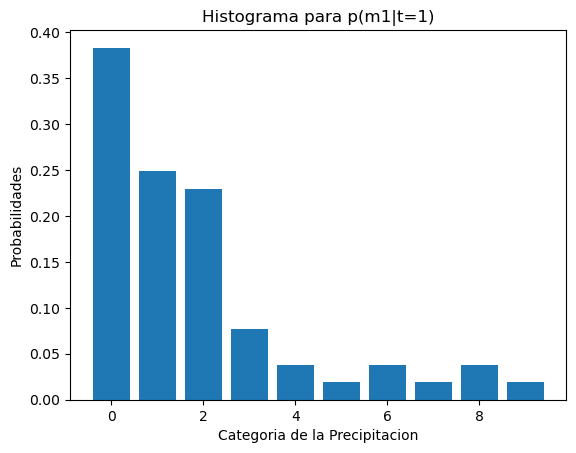
\includegraphics[width=0.75\linewidth]{Quiz_2//Imagenes/histograma_precipitacion_t1.png}
    \caption{Histograma para la precipitaci\'{on} cuando $t = 1$}
    \label{fig:hist_precipitacion_t1}
\end{figure}

\selectlanguage{spanish}%
\begin{figure}[hbtp!]
    \centering
    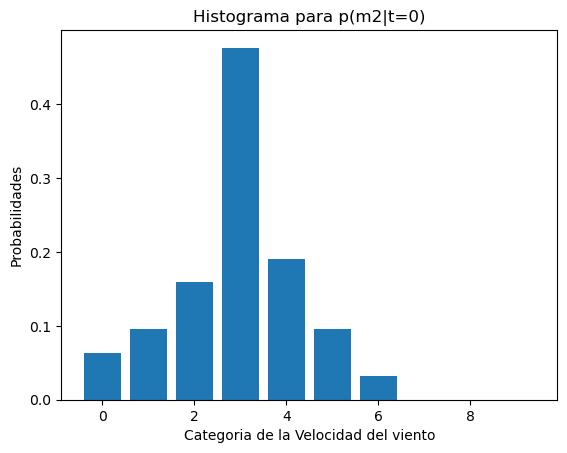
\includegraphics[width=0.75\linewidth]{Quiz_2//Imagenes/histograma_viento_t0.png}
    \caption{Histograma para la velocidad del viento cuando $t = 0$}
    \label{fig:hist_viento_t0}
\end{figure}\newpage

\selectlanguage{spanish}%
\begin{figure}[hbtp!]
    \centering
    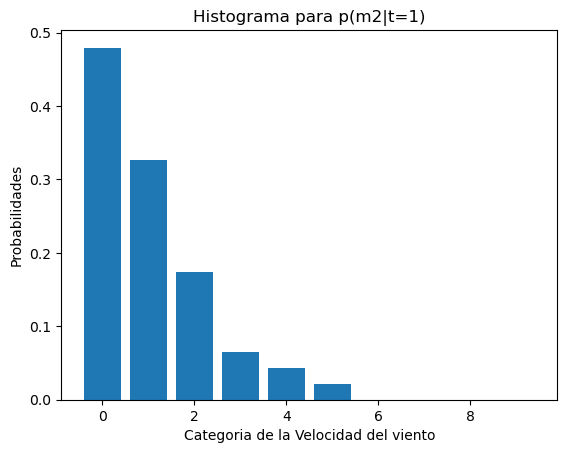
\includegraphics[width=0.75\linewidth]{Quiz_2//Imagenes/histograma_viento_t1.png}
    \caption{Histograma para la velocidad del viento cuando $t = 1$}
    \label{fig:hist_viento_t1}
\end{figure}

Como conclusiones en este punto tenemos:
\begin{enumerate}
    \item La distribuci\'{o}n que sugiere la figura \ref{fig:hist_precipitacion_t0} es \textbf{Gaussiana}.
    \item La distribuci\'{o}n que sugiere la figura \ref{fig:hist_precipitacion_t1} es \textbf{Exponencial}.
    \item La distribuci\'{o}n que sugiere la figura \ref{fig:hist_viento_t0} es \textbf{Gaussiana}.
    \item La distribuci\'{o}n que sugiere la figura \ref{fig:hist_viento_t1} es \textbf{Exponencial}.
\end{enumerate}

\item \textbf{(50 puntos)} Utilizando los graficos anteriores, ajuste un
modelo Gaussiano o exponencial, segun sea necesario (realice la justificacion
segun lo observado en tales graficos), a cada una de las densidades
$p\left(m_{1}|t=0\right)$, $p\left(m_{1}|t=1\right),$$p\left(m_{2}|t=0\right)$,
$p\left(m_{2}|t=1\right)$. Muestre los pasos intermedios para estimar
los parametros de tales modelos y documentelos. Grafique el modelo
ajustado y muestre las tablas \foreignlanguage{english}{\ref{tab:Datos-para-la-P}
y \ref{tab:Datos-para-la-P-1}} con las probabilidades estimadas por
estos nuevos modelos.

Se crearon dos funciones para poder modelar tanto de forma Gaussiana como Exponencial:

\textbf{Funci\'{o}n del modelo Gaussiano:} Este recibe como entradas el valor a evaluar (data), la media $\mu$ (mean) y la desviaci\'{o}n estandar $\sigma$ (sigma), y retorna el valor de la probabilidad gaussiana. La ecuaci\'{o}n modelada es la siguiente:

\begin{equation}
    p\left(x\right)=\frac{1}{\sqrt{2\pi\sigma^{2}}}e^{\frac{-1}{2}\left(\frac{x-\mu}{\sigma}\right)^{2}}
\end{equation}\label{eq:func_prob_gauss}

\begin{lstlisting}[language=Python]
def gauss_model(data,mean,sigma):
    fraction = 1/((torch.sqrt(torch.tensor(2 * torch.pi * sigma**2))))
    exponential = torch.exp(torch.tensor((-1/2) * ((data - mean)/sigma)**2))
    prob_gauss = fraction * exponential
    return prob_gauss
\end{lstlisting}

\textbf{Funci\'{o}n del modelo Exponencial:} Este recibe como entradas el valor a evaluar (data) y el $\lambda$ (lambda\_dist). La ecuaci\'{o}n modelada es la siguiente:

\begin{equation}
    p\left(x\right)=\lambda e^{-\lambda x}
\end{equation}\label{eq:func_prob_exp}

\begin{lstlisting}[language=Python]
def exp_model(data,lambda_dist):
    prob_exp = lambda_dist * torch.exp(torch.tensor(-lambda_dist * data))
    return prob_exp
\end{lstlisting}

A continuaci\'{o}n se explica el proceso de selecci\'{o}n de los par\'{a}metros $\mu$, $\sigma$ y $\lambda$ dependiendo del caso. Adem\'{a}s, los datos evaluados en las funciones son 1000 puntos que van de 0 a 9, para tener una l\'{i}nea clara que permita seleccionar los par\'{a}metros m\'{a}s f\'{a}cilmente.

\begin{enumerate}
    \item \textbf{Funci\'{o}n de densidad de probabilidad Gaussiana para la variable aleatoria P cuando t=0}: Como se observa en el histograma, la media est\'{a} alrededor de los 7. Ya con ese valor seleccionado, se paso a probar diferentes valores de desviaci\'{o}n est\'{a}ndar para que la curva reflejara un comportamiento que emulara de forma acertada el histograma. Dicho valor de $\sigma$ termin\'{o} siendo 3.

    \selectlanguage{spanish}%
    \begin{figure}[hbtp!]
        \centering
        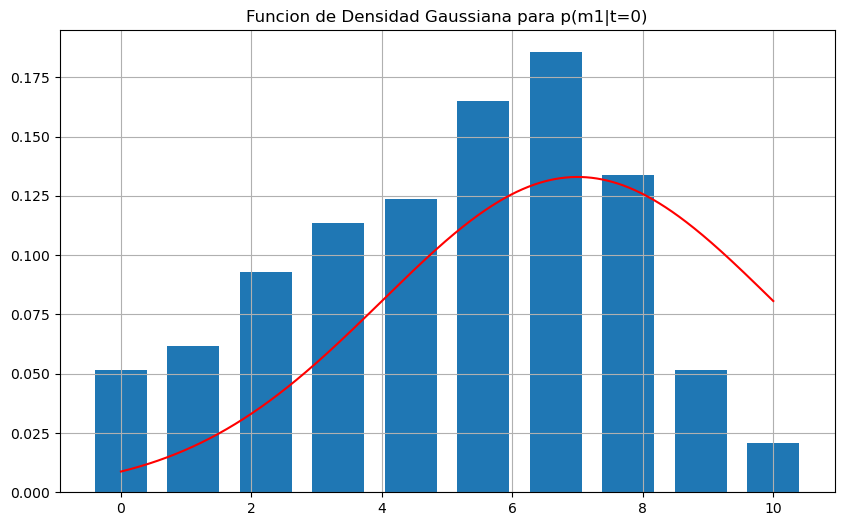
\includegraphics[width=0.75\linewidth]{Quiz_2//Imagenes/pdf_precipitacion_t0.png}
        \caption{Histograma y funci\'{o}n de densidad de probabilidad Gaussiana para la variable aleatoria P cuando t=0.}
        \label{fig:hist_pdf_p_t0}
    \end{figure}\newpage

    \item \textbf{Funci\'{o}n de densidad de probabilidad Exponencial para la variable aleatoria P cuando t=1}: Para este caso, se probaron diferentes valores de $\lambda$ hasta encontrar uno que generara una l\'{i}nea que describiera bien el histograma. El valor seleccionado al final de $\lambda$ fue de 0.4.

    \selectlanguage{spanish}%
    \begin{figure}[hbtp!]
        \centering
        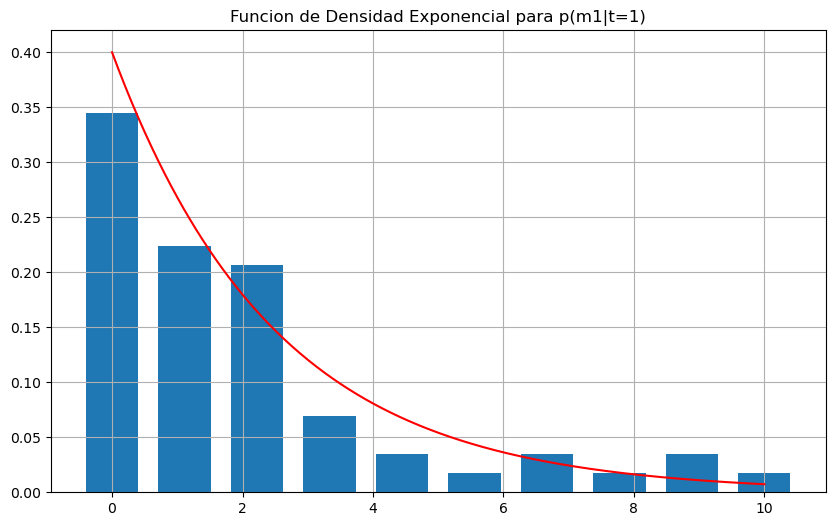
\includegraphics[width=0.75\linewidth]{Quiz_2//Imagenes/pdf_precipitacion_t1.png}
        \caption{Histograma y funci\'{o}n de densidad de probabilidad Exponencial para la variable aleatoria P cuando t=1.}
        \label{fig:hist_pdf_p_t1}
    \end{figure}\newpage

    \item \textbf{Funci\'{o}n de densidad de probabilidad Gaussiana para la variable aleatoria V cuando t=0}: De la misma forma que con la variable aleatoria P, se determin\'{o} que la media est\'{a} alrededor de 3.5 (despu\'{e}s de varias iteraciones se concluy\'{o} que 3.4 funciona mejor). Luego se paso a probar diferentes valores de desviaci\'{o}n est\'{a}ndar para que la curva reflejara un comportamiento que emulara de forma acertada el histograma. Dicho valor de $\sigma$ termin\'{o} siendo 1.3, el cual castiga un poco la categor\'{i}a cero, pero es una condici\'{o}n aceptable por la naturaleza de los datos.

    \selectlanguage{spanish}%
    \begin{figure}[hbtp!]
        \centering
        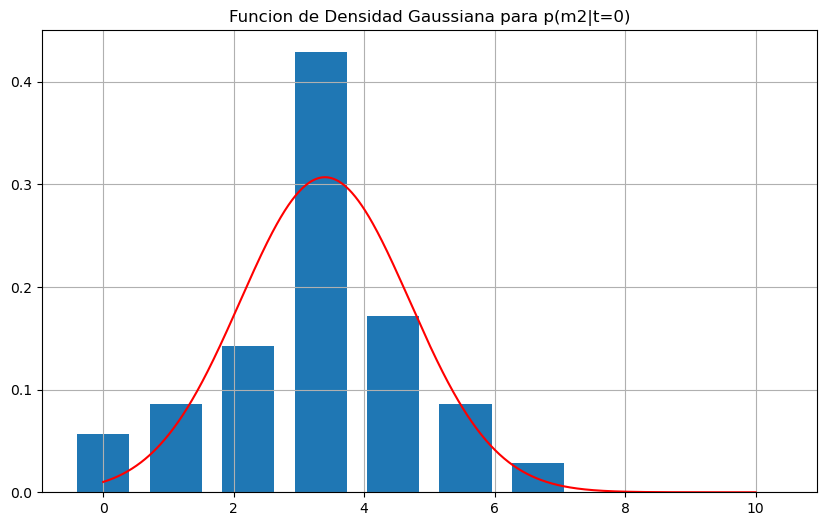
\includegraphics[width=0.75\linewidth]{Quiz_2//Imagenes/pdf_viento_t0.png}
        \caption{Histograma y funci\'{o}n de densidad de probabilidad Gaussiana para la variable aleatoria V cuando t=0.}
        \label{fig:hist_pdf_v_t0}
    \end{figure}\newpage

    \item \textbf{Funci\'{o}n de densidad de probabilidad Exponencial para la variable aleatoria V cuando t=1}: Igual que para la variable aleatorio P, se probaron diferentes valores de $\lambda$ hasta encontrar uno que generara una l\'{i}nea que describiera bien el histograma. El valor seleccionado al final de $\lambda$ fue de 0.5.

    \selectlanguage{spanish}%
    \begin{figure}[hbtp!]
        \centering
        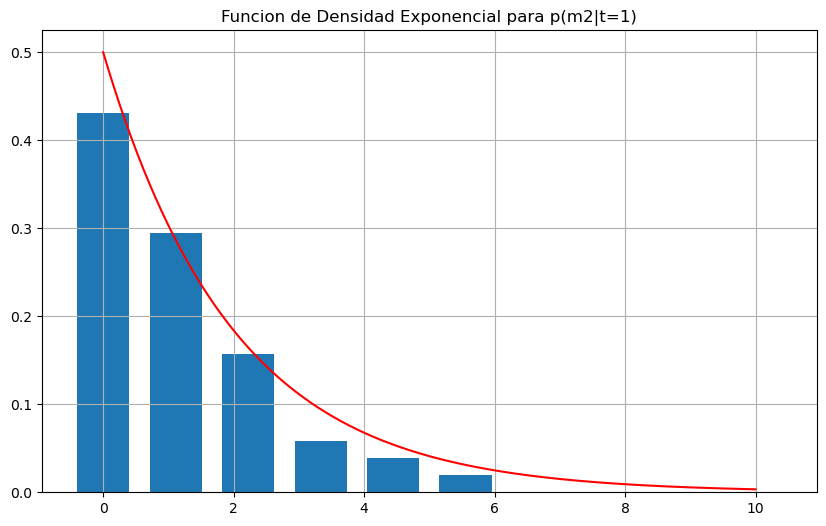
\includegraphics[width=0.75\linewidth]{Quiz_2//Imagenes/pdf_viento_t1.png}
        \caption{Histograma y funci\'{o}n de densidad de probabilidad Exponencial para la variable aleatoria v cuando t=1.}
        \label{fig:hist_pdf_v_t1}
    \end{figure}
    
\end{enumerate}

Los c\'{o}digos usados para poder crear estas figuras fueron los siguientes (fueron siendo ajustados dependiendo del caso de estudio):

\textbf{Para el modelo Gaussiano:}
\begin{lstlisting}[language=Python]
# Funcion de densidad de probabilidad gaussiana de p(m1|t=0)
# Medias y desviacion estandar
p_m1_t0_mean = 7
p_m1_t0_std = 3


# Eje x de la funcion gaussiana
x = np.linspace(0, 10, 1000)

# Creando la funcion de densidad gaussiana
prob_m1_t0_densfunct = gauss_model(x,p_m1_t0_mean,p_m1_t0_std)

# Acomondando los bines para que empiecen en cero
bins = torch.linspace(0, 10, 10)

# Plot the density function
plt.figure(figsize=(10, 6))
histogram,bins_hist = torch.histogram(bins,bins=10,weight=P[0,:], density=True)
plt.bar(bins,histogram)
plt.plot(x, prob_m1_t0_densfunct, label=f'Funcion Gaussiana 1', color='red')
plt.title('Funcion de Densidad Gaussiana para p(m1|t=0)')
plt.grid(True)
plt.show()istograma para p(m1|t=0)')
plt.show()
\end{lstlisting}

\textbf{Para el modelo Exponencial:}
\begin{lstlisting}[language=Python]
# Funcion de densidad de probabilidad exponencial de p(m1|t=0)
# Lambda para la funcion exponencial
p_m1_t1_lambda = 0.4

# Eje x de la funcion exponencial
x = np.linspace(0, 10, 1000)

# Acomondando los bines para que empiecen en cero
bins = torch.linspace(0, 10, 10)

# Calculando la funcion exponencial
expo = exp_model(x,p_m1_t1_lambda)

# Ploteando la funcion de densidad con el histograma
plt.figure(figsize=(10, 6))
histogram,bins_hist = torch.histogram(bins,bins=10,weight=P[1,:], density=True)
plt.bar(bins,histogram)
plt.plot(x, expo, label=f'Funcion exponencial 1', color='red')
plt.title('Funcion de Densidad Exponencial para p(m1|t=1)')
plt.grid(True)
plt.show()
\end{lstlisting}\newpage

Por \'{u}ltimo, ya con todos los modelos creados, se procedi\'{o} a calcular las nuevas probabilidades para todas las categor\'{i}as de las variables aleatorias. Las siguientes dos tablas muestran estos resultados:

\selectlanguage{spanish}%
\begin{table}[hbtp!]
    \centering
    \begin{tabular}{|c|c|c|c|c|c|c|c|c|c|c|}
    \hline 
         &$p=400$&$p=500$&$p=600$&$p=700$&$p=800$&$p=900$&$p=1000$&$p=1100$&$p=1200$&$p=1300$\\
    \hline 
         $t=0$& 0.0087&0.0194&0.0374&0.0630&0.0925&0.1184&0.1322&0.1286&0.1091&0.0807\\
    \hline 
         $t=1$&0.4000&0.2565&0.1644&0.1054&0.0676&0.0433&0.0278&0.0178&0.0114&0.0073\\
    \hline 
    \end{tabular}
    \caption{Probabilidad de la variable aleatoria P, calculados con los modelos Gaussiano y Exponencial}
    \label{tab:prob_P}
\end{table}

\selectlanguage{spanish}%
\begin{table}[hbtp!]
    \centering
    \begin{tabular}{|c|c|c|c|c|c|c|c|c|c|c|}
    \hline 
         &$v=5$&$v=10$&$v=15$&$v=20$&$v=25$&$v=30$&$v=35$&$v=40$&$v=45$&$v=50$\\
    \hline 
         $t=0$&1.00e-02&6.51e-02&2.03e-01&3.06e-01&2.22e-01&7.76e-02&1.30e-02&1.05e-03&4.12e-05&7.76e-07\\
    \hline 
         $t=1$&5.00e-01&2.86e-01&1.64e-01&9.44e-02&5.41e-02&3.10e-02&1.78e-02&1.02e-02&5.87e-03&3.36e-03\\
    \hline 
    \end{tabular}
    \caption{Probabilidad de la variable aleatoria V, calculados con los modelos Gaussiano y Exponencial}
    \label{tab:prob_V}
\end{table}

Las tablas \ref{tab:prob_P} y \ref{tab:prob_V} fueron populadas con el siguiente c\'{o}digo:

\begin{lstlisting}[language=Python]
# Creando los tensores con las probabilidades
prob_P = torch.zeros([2,10])
prob_V = torch.zeros([2,10])

# Creando los bines que van a ser evaluados en las funciones
bins = np.linspace(0,10,10)

# Probabilidades para p(m=1|t=0)
p_m1_t0 = gauss_model(bins,p_m1_t0_mean,p_m1_t0_std)
prob_P[0,:] = p_m1_t0

# Probabilidades para p(m=1|t=1)
p_m1_t1 = exp_model(bins,p_m1_t1_lambda)
prob_P[1,:] = p_m1_t1

# Probabilidades para p(m=1|t=0)
p_m2_t0 = gauss_model(bins,p_m2_t0_mean,p_m2_t0_std)
prob_V[0,:] = p_m2_t0

# Probabilidades para p(m=1|t=0)
p_m2_t1 = exp_model(bins,p_m2_t1_lambda)
prob_V[1,:] = p_m2_t1

# Imprimiendo los resultados
print("Probabilidad de p=m1:\n", prob_P)
print("Probabilidad de v=m2:\n", prob_V)
\end{lstlisting}

\item \textbf{(30 puntos)} Usando Bayes, estime si habra corte electrico
para una entrada $m_{1}=500$ y $m_{2}=10$. Muestre y explique los
pasos intermedios.\selectlanguage{english}%

En la secci\'{o}n \textit{1.4 Bayes ingenuo y regresi\'{o}n log\'{i}stica} de \cite{Calderon_Clasificacion_Binaria} se explica c\'{o}mo la verosimilitud tiene una relaci\'{o}n proporcional explicada en la siguiente ecuaci\'{o}n:

\begin{equation}\label{eq:bayes_ingenuo_general}
p\left(t=k|\overrightarrow{m}\right)\propto\prod_{i=0}^{D}p\left(m_{d}|t=k\right)p\left(t=k\right)
\end{equation}

Para el desarrollo de este quiz, se desarroll\'{o} \ref{eq:bayes_ingenuo_general} para obtener la siguiente ecuaci\'{o}n:

\begin{equation}\label{eq:bayes_ingenuo_quiz}
p\left(t|m_{1},m_{2}\right) = p\left(m_{1}|t\right)p_{m1}\left(t\right)p\left(m_{2}|t\right)p_{m2}\left(t\right)
\end{equation}

Para poder crear una funci\'{o}n de \ref{eq:bayes_ingenuo_quiz}, es necesario una funci\'{o}n intermedia para calcular la probabilidad a priori para cada una de las variables aleatorias.

El siguiente c\'{o}digo calcula la probabilidad a priori para cada una de las variables aleatorias, el cual recibe como entrada una de las tablas \ref{tab:prob_P} o \ref{tab:prob_V} dependiendo del caso:

\begin{lstlisting}[language=Python]
def prob_a_priori(data):
    data_t_0 = data[0,:]
    data_t_1 = data[1,:]
    
    N = torch.sum(data)
    
    return torch.tensor([[torch.sum(data_t_0)/N],[torch.sum(data_t_1)/N]])
\end{lstlisting}

Al ejecutar esta funcion con las tablas \ref{tab:prob_P} y \ref{tab:prob_V} se obtiene los siguientes valores:

\begin{lstlisting}[language=Python]
# Calculando el tensor con los probabilidades a priori de m1
p_priori_m1 = prob_a_priori(prob_P)
print("Probabilidad a priori para P:\n",p_priori_m1)

# Calculando el tensor con los probabilidades a priori de m2
p_priori_m2 = prob_a_priori(prob_V)
print("Probabilidad a priori para V:\n",p_priori_m2)

Resultados impresos:
Probabilidad a priori para P:
 tensor([[0.4176],
        [0.5824]])
Probabilidad a priori para V:
 tensor([[0.4349],
        [0.5651]])
\end{lstlisting}

Ahora se puede crear la siguiente funci\'{o}n para \ref{eq:bayes_ingenuo_quiz}:

\begin{lstlisting}[language=Python]
def predecir_evento(va_P_index,va_V_index,value_t,prob_va_P,prob_va_V,prob_t_m1,prob_t_m2):
    # Primera variable aleatoria
    p_m_t_m1 = prob_va_P[value_t,va_P_index]
    p_t_m1 = prob_t_m1[value_t]
    
    # Segunda variable aleatoria
    p_m_t_m2 = prob_va_V[value_t,va_V_index]
    p_t_m2 = prob_t_m2[value_t]
    
    bayes_ingenuo = p_m_t_m1 * p_t_m1 * p_m_t_m2 * p_t_m2
    return bayes_ingenuo
\end{lstlisting}

Con esta funci\'{o}n ya creada, se procede un c\'{o}digo que realiza la siguiente l\'{o}gica:

\begin{enumerate}
    \item Escoger la clase de cada variable aleatoria a ser evaluada.
    \item Usando la funci\'{o}n \textit{predecir\_evento} (que corre Bayes ingenuo), correr tanto para el escenario t = 0 (NO es necesario hacer un corte el\'{e}ctrico) y t = 1 (SI es necesario hacer un corte el\'{e}ctrico).
    \item Finalmente, comprar tanto el evento t0 contra el t1, determinar cual tiene mayor verosimilitud, y concluir si es necesario hacer un corte el\'{e}ctrico o no.
\end{enumerate}

A continuaci\'{o}n se presenta el c\'{o}digo explicado anteriormente:

\begin{lstlisting}[language=Python]
# Indicadores de la variable aleatoria
P_index = 1 # 1 Corresponde a p = 500 l/m^2
V_index = 1 # 1 Corresponde a v = 10 km/h

# Calculando Bayes para t=0
t = 0
evento_t0 = predecir_evento(P_index,V_index,t,prob_P,prob_V,p_priori_m1,p_priori_m2)
print("Verosimilitud del evento t=0\n",evento_t0)

# Calculando Bayes para t=1
t = 1
evento_t1 = predecir_evento(P_index,V_index,t,prob_P,prob_V,p_priori_m1,p_priori_m2)
print("Verosimilitud del evento t=1\n",evento_t1)

# Por ultimo, se calcula si hay que racionar, donde t = 0 es NO RACIONAR y t = 1 es RACIONAR
print("\nDecision:")
if(evento_t0 > evento_t1):
    print("NO es necesario hacer un corte electrico!")
if(evento_t0 <= evento_t1):
    print("SI es necesario hacer un corte electrico!")
\end{lstlisting}

Que al ser ejecutado para $p=500l/m^2$ (clase \#1 para la variable aleatorio P) y $v=10km/h$ (clase \#1 para la variable aleatorio V) se obtiene la siguiente respuesta:

\begin{lstlisting}[language=Python]
Verosimilitud del evento t=0
 tensor([0.0002])
Verosimilitud del evento t=1
 tensor([0.0242])

Decision:
SI es necesario hacer un corte electrico!
\end{lstlisting}

Y por lo tanto, se concluye que \textbf{SI es necesario} hacer un corte el\'{e}ctrico cuando $p=500l/m^2$ y $v=10km/h$.

\end{enumerate}

\printbibliography[
heading=bibintoc,
title={Bibliograf\'{i}a}
]

\end{document}
